\documentclass[a4paper]{scrreprt}

\usepackage[german]{babel}
\usepackage[utf8]{inputenc}
\usepackage[T1]{fontenc}
\usepackage{ae}
\usepackage[bookmarks,bookmarksnumbered]{hyperref}
\usepackage{graphicx}
\usepackage[toc]{glossaries}
\usepackage{float}
\usepackage{listings}

\graphicspath{ {Images/} }
\setcounter{secnumdepth}{5}
\makeglossaries

\begin{document}
    \def\code#1{\texttt{#1}}

    \begin{flushright}
        
\includegraphics[scale = 0.7]{kit-logo.jpg}\\[0.5cm]
        % 
\includegraphics[scale = 1]{teco.jpg}
    \end{flushright}
    % 
\includegraphics[scale = 0.5]{kit-logo.jpg} \hspace{4cm} 
\includegraphics[scale = 1]{teco.jpg}
    \vspace*{2cm}

    \begin{center} \large

        Praxis der Softwareentwicklung
        \vspace * {1.5cm}

        \textbf{\huge Mind Rate}

        \vspace*{1cm}


        {\Large Ein interaktives System mit Android-Client f\"ur Studien nach Experience-Sampling-Method (ESM)}

        \vspace*{1cm}

        \textbf{\Large Entwurf}
        \vspace*{2cm}

        Shanshan Du, Yi Ge, Renhan Lou, Ruoheng Ma, Haobin Tan
        \vspace*{1cm}

        02. Dezember 2016
        \vspace*{2.5cm}

        Betreuung: Anja Exler, Dr. Andrea Schankin\\[0.5cm]
        Forschungsgruppe TECO: Technology for Pervasive Computing\\[0.5cm]

        Karlsruher Institut für Technologie
    \end{center}
    \thispagestyle{empty}

    \tableofcontents

    \chapter{Allgemeine Struktur}

        Der Entwurf besteht aus zwei Seiten: der Android-App-Seite und der Server-Seite. Sie sind jeweils für die Android-App und das Web-Interface verantwortlich. Zusätzlich soll eine Datenbank auf dem Server laufen, um alle Studien-, Konto- und Probandendaten zu speichern. Diese gehört auch zu der Server-Seite. Die zwei Seiten sollen miteinander durch das HTTP-Protokoll kommunizieren.

    \chapter{Server-Seite}
        Die Server-Seite nutzt eine von Django-Framework veränderte Variante\footnote{\href{https://docs.djangoproject.com/en/1.10/faq/general/\#django-appears-to-be-a-mvc-framework-but-you-call-the-controller-the-view-and-the-view-the-template-how-come-you-don-t-use-the-standard-names}{https://docs.djangoproject.com/en/1.10/faq/general/\#django-appears-to-be-a-mvc-framework-but-you-call-the-controller-the-view-and-the-view-the-template-how-come-you-don-t-use-the-standard-names}} der Modell-Präsentation-Steuerung-Architektur (MVC) als den Architekturstil. Die benötigte Klassen werden als Modelle entworfen. Der Entwurf von Server-Seite wird auf Python angefertigt.

        \section{Modelle}
            \begin{itemize}
                \item \code{class StudyDirector}
                    \begin{itemize}
                        \item \code{studies = []: Study}
                        \item \code{surname}
                        \item \code{firstName}
                        \item \code{mailAddress}
                    \end{itemize}

                    \item \code{class Study}
                        \begin{itemize}
                            \item \code{probands = []: Proband}
                            \item \code{id}
                            \item \code{name}
                            \item \code{beginningDate}
                            \item \code{endDate}
                            \item \code{director: StudyDirector}
                            \item \code{questionnaires = []: Questionnaire}
                        \end{itemize}

                    \item \code{class Proband}
                        \begin{itemize}
                            \item \code{study: Study}
                            \item \code{id}
                            \item \code{birthday}
                            \item \code{occupation}
                            \item \code{gender}
                        \end{itemize}

                    \item \code{class Questionnairer}
                        \begin{itemize}
                            \item \code{questions = []: AbstractQuestion}
                            \item \code{id}
                            \item \code{name}
                            \item \code{study: Study}
                            \item \code{triggerEvent: TriggerEvent}
                            \item \code{answeringTime}
                            \item \code{answers = []: QuestionnaireAnswer}
                        \end{itemize}

                    \item \code{class QuestionnaireAnswer}
                        \begin{itemize}
                            \item \code{submitter: Proband}
                            \item \code{submitTime}
                            \item \code{questionAnswers = []: AbstractQuestionAnswer}
                        \end{itemize}

                    \item \code{class AbstractQuestion(ABC)}
                        \begin{itemize}
                            \item \code{id}
                            \item \code{questionnaire: Questionnaire}
                        \end{itemize}

                    \item \code{class TextQuestion(AbstractQuestion)}
                        \begin{itemize}
                            \item \code{content}
                        \end{itemize}

                    \item \code{class ChoiceQuestion(AbstractQuestion)}
                        \par // Both single choice question and multiple choice question are belonging to this class.
                        \begin{itemize}
                            \item \code{options = \{\}}
                            \item \code{followUpQuestion: AbstractQuestion}
                            \item \code{followUpQuestionTriggerOptions = []}
                        \end{itemize}

                    \item \code{class SteplessScaleQuestion(AbstractQuestion)}
                        \par // Scale questions with steps are effectively just single choice questions; therefore they are not a class.
                        \begin{itemize}
                            \item \code{scaleMin: int}
                            \item \code{scaleMax: int}
                            \item \code{followUpQuestion: AbstractQuestion}
                            \item \code{followUpQuestionTriggerMin: int}
                            \item \code{followUpQuestionTriggerMax: int}
                        \end{itemize}

                    \item \code{class AbstractQuestionAnswer(ABC)}
                        \begin{itemize}
                            \item \code{content}
                        \end{itemize}

                   \item \code{class TextQuestionAnswer(AbstractQuestionAnswer)}
                       \begin{itemize}
                           \item \code{content: string}
                       \end{itemize}

                   \item \code{class MultiChoiceQuestionAnswer(AbstractQuestionAnswer)}
                       \begin{itemize}
                           \item \code{content = []: string}
                       \end{itemize}

                    \item \code{class SingleChoiceQuestionAnswer(AbstractQuestionAnswer)}
                        \begin{itemize}
                            \item \code{content: string}
                        \end{itemize}

                    \item \code{class SteplessScaleQuestionAnswer(AbstractQuestionAnswer)}
                        \begin{itemize}
                            \item \code{content: int}
                        \end{itemize}

            \end{itemize}

        \newpage
        \section{Entity-Relationship-Modell der Datenbank}
            \begin{figure}[ht]
                \centering
                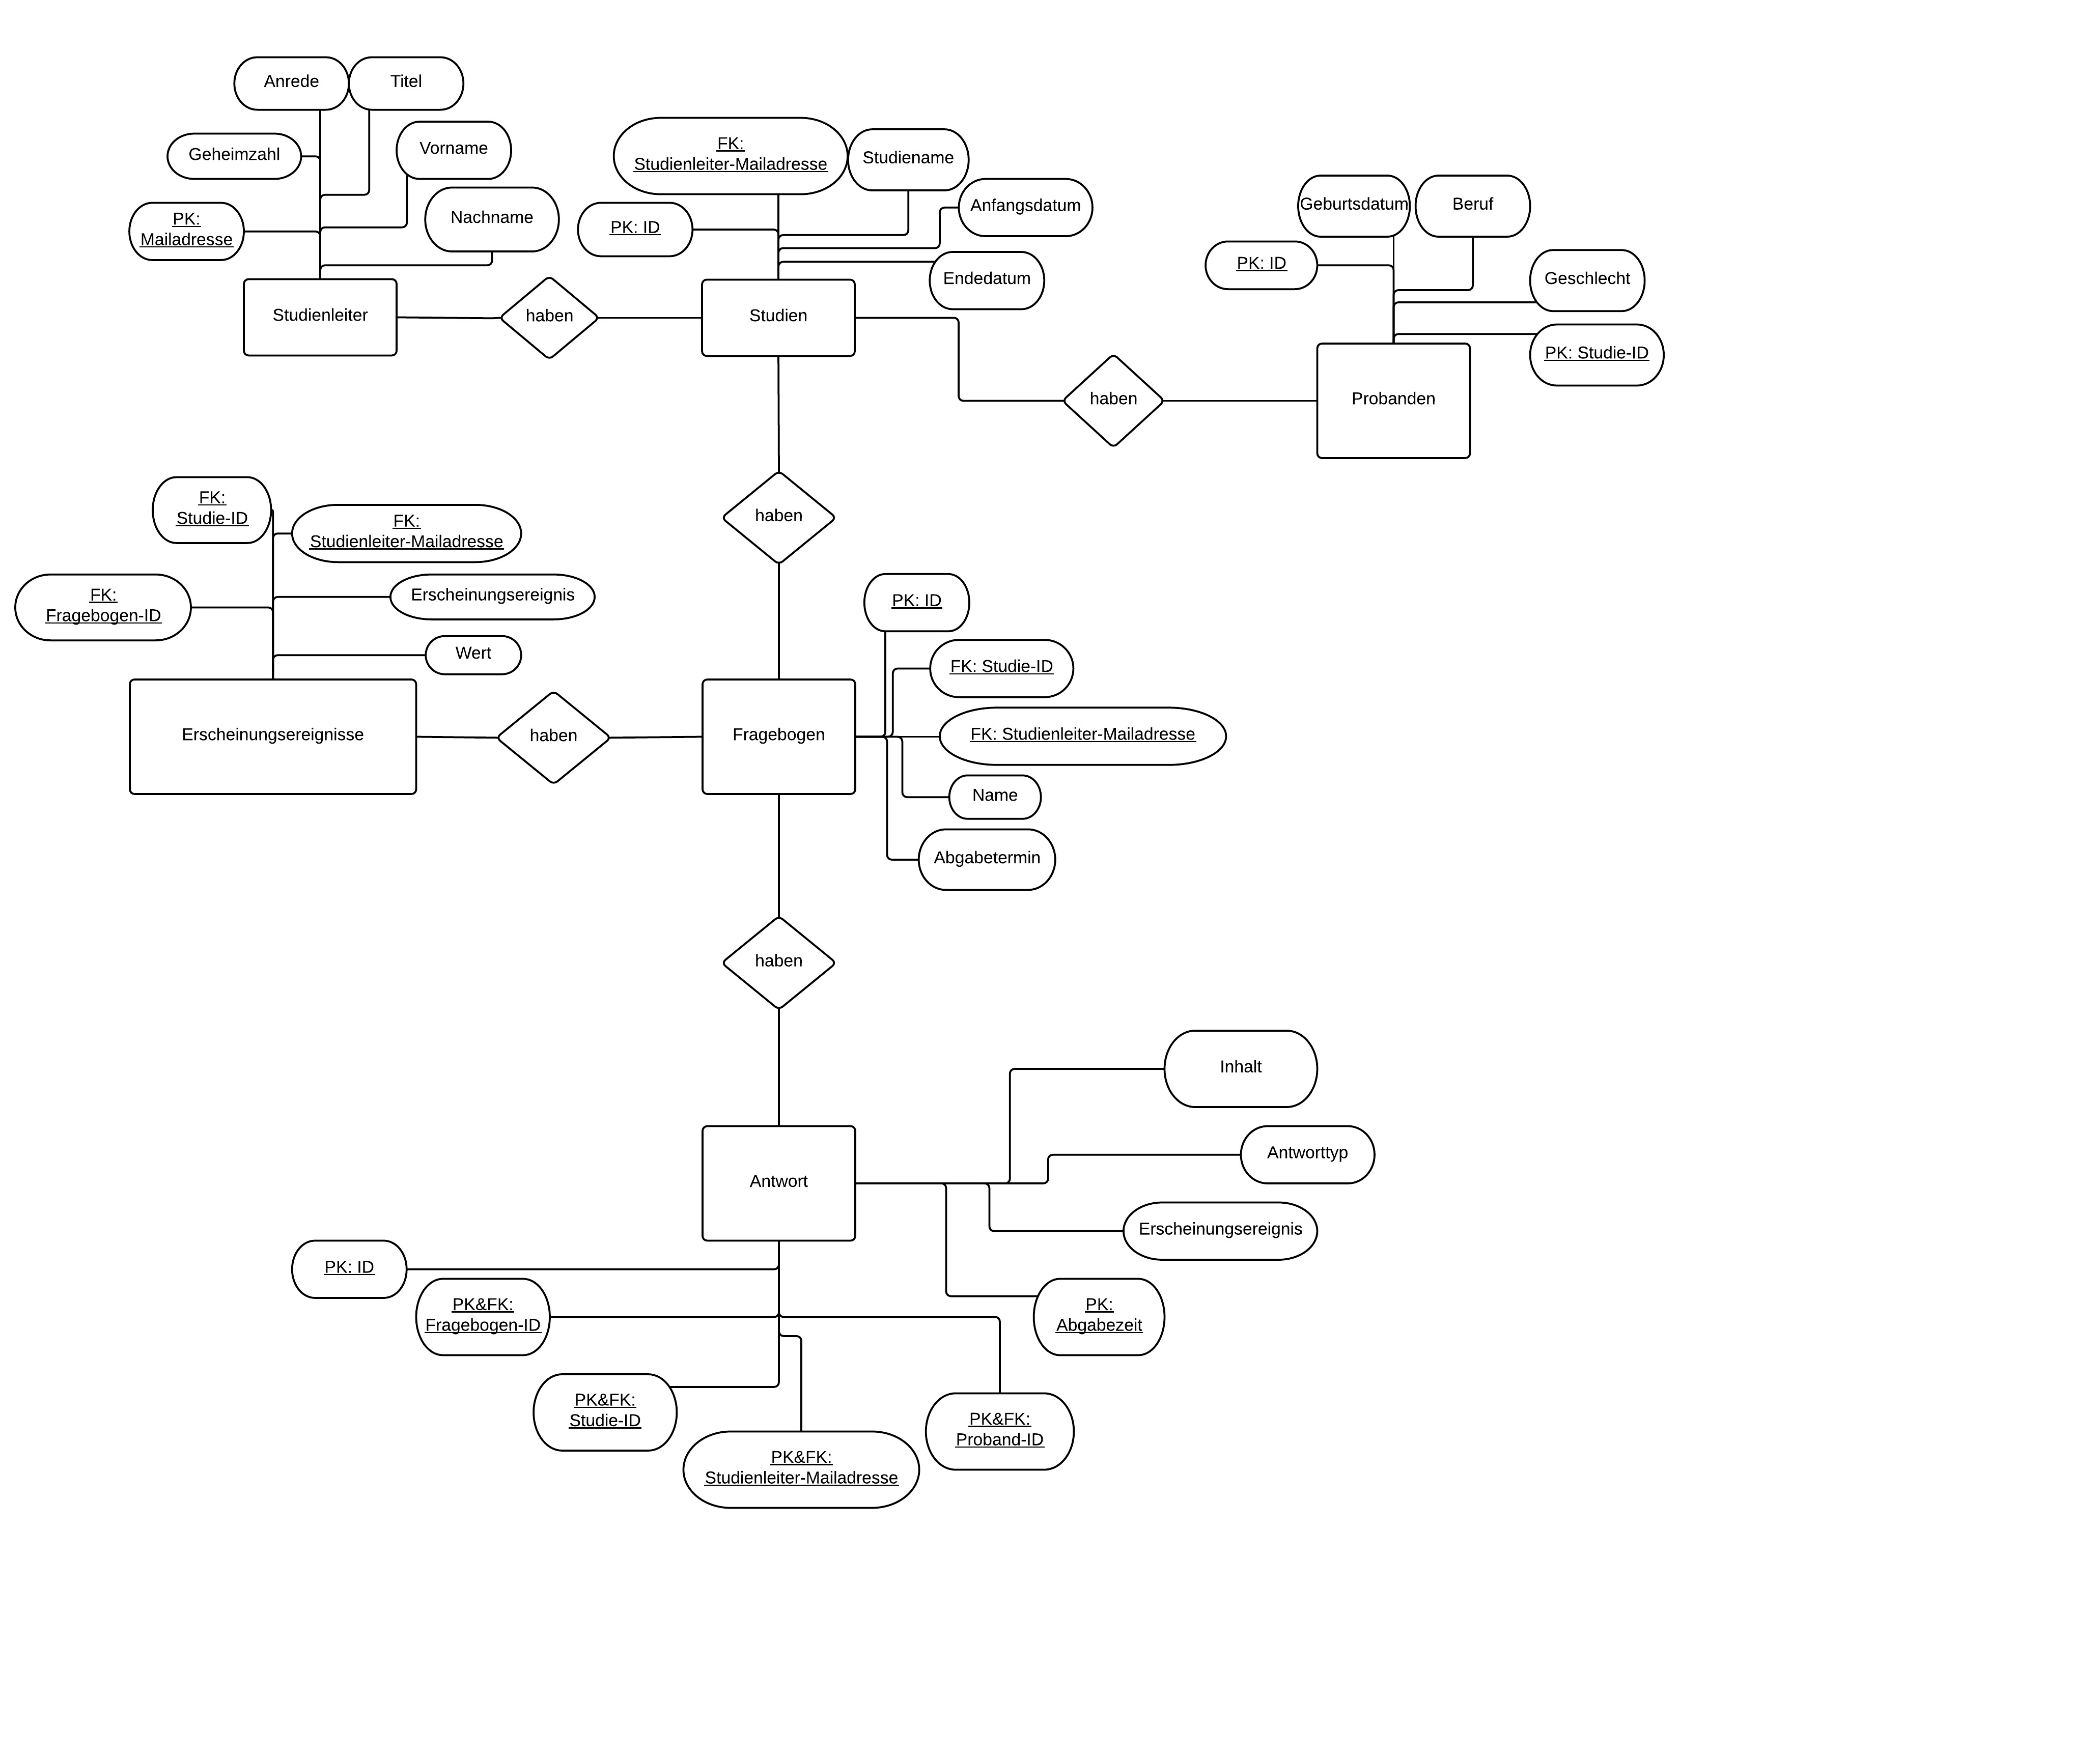
\includegraphics[scale = 0.13]{PSE_Datenbank_ERM.jpeg}
                \caption{Entity-Relationship-Modell der Datenbank}
            \end{figure}


    \newpage
    \chapter{Android-App}

        Das Entwurfsmuster Model-View-Controller (MVC, englisch für Modell-Präsentation-Steuerung) wird hier eingesetzt, um einen fleixbler Programmentwurf zu ermöglichen.


        \vspace*{1cm}
        \section{Überblick von Pakete}

            Das folgende Diagramm dient sich als einen Überblick über unsere Android App. Modell, Präsentation udn Steuerung werden mit drei verschiedenen Farbe dargestellt: blau für Modell, grün für Präsentation und gelb für Steuerung.

            \noindent Um die Beziehungen zwischen Klassen und das System ganzheitlich aufzufassen, enthält folgendes Diagramm keine Attribute und Methoden. Jede Pakete sowie Klasse mit Attribute und Methoden werden dann ausführlich beschreiben.



            \newpage
            \vspace*{1cm}
            \begin{figure}[H]
                \centering
                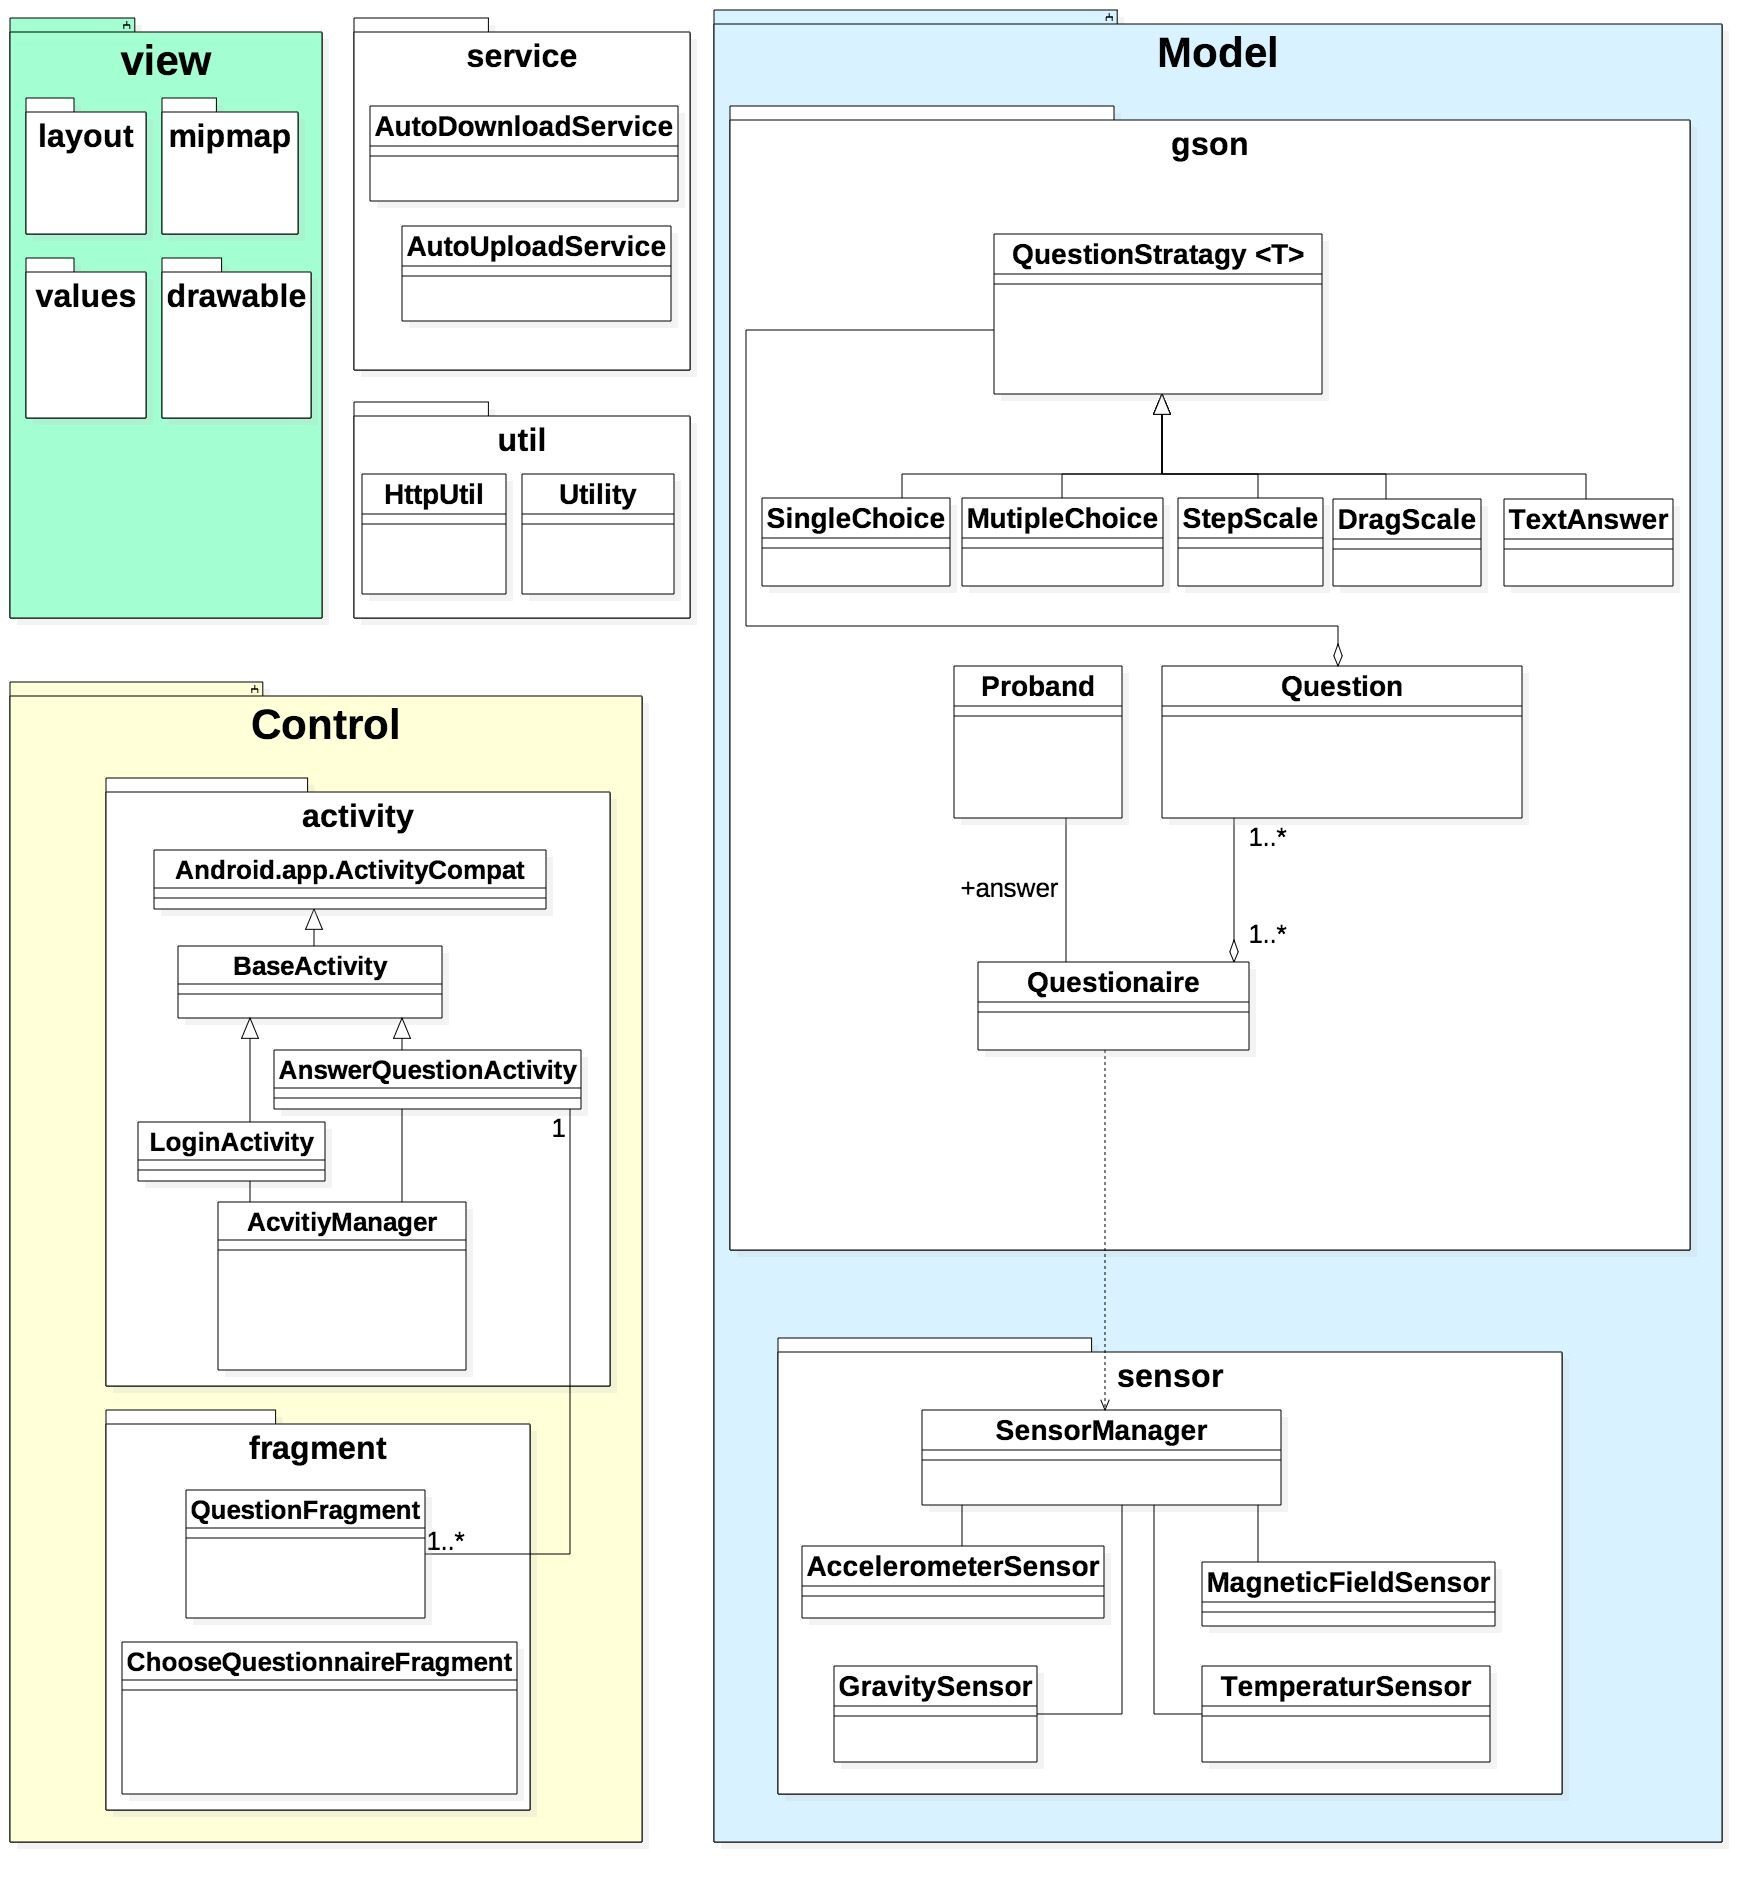
\includegraphics[scale = 0.25]{packageDiagram.jpg}
                \caption{Überblick über alle Packte und Klasse (ohne Attribute und Methoden)}
            \end{figure}




        %TODO: Ausführliche Beschreibung für jedes package und klasse davon

        \section{Model}

            Der Teil Model besteht aus zwei Pakete: gson und sensor.

            \begin{figure}[H]
                \centering
                % 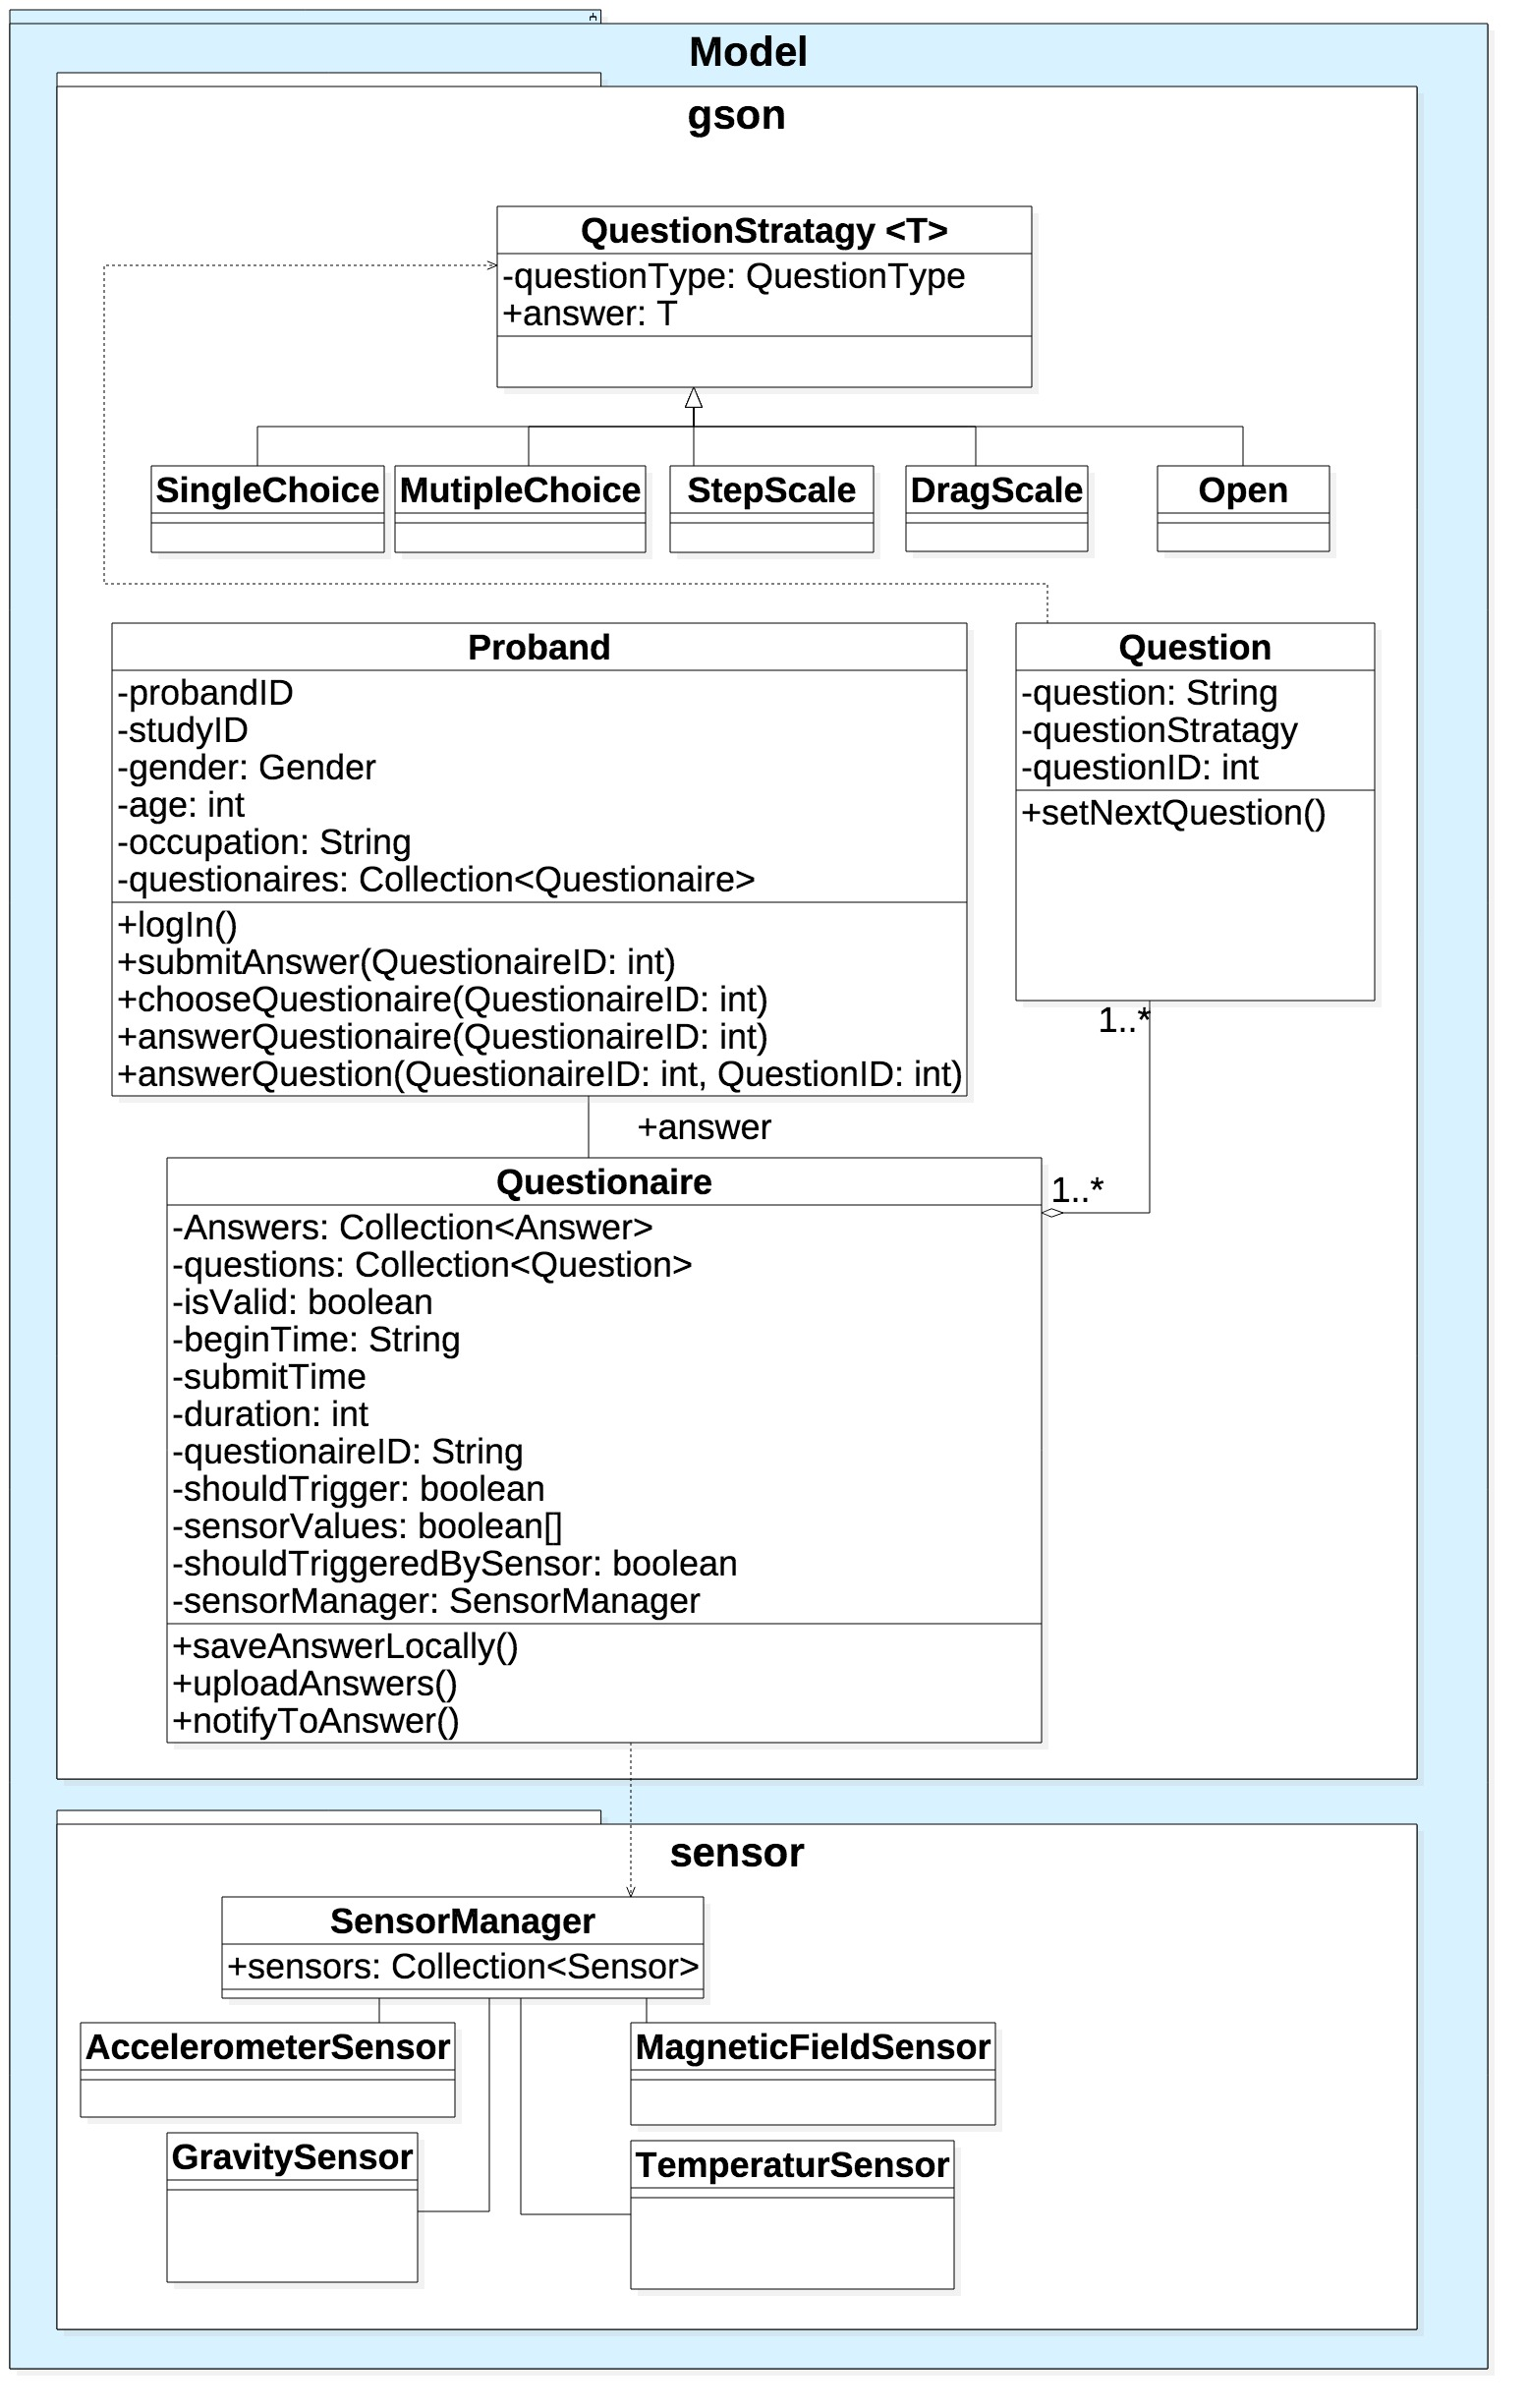
\includegraphics[scale = 0.25]{Model.jpg}
                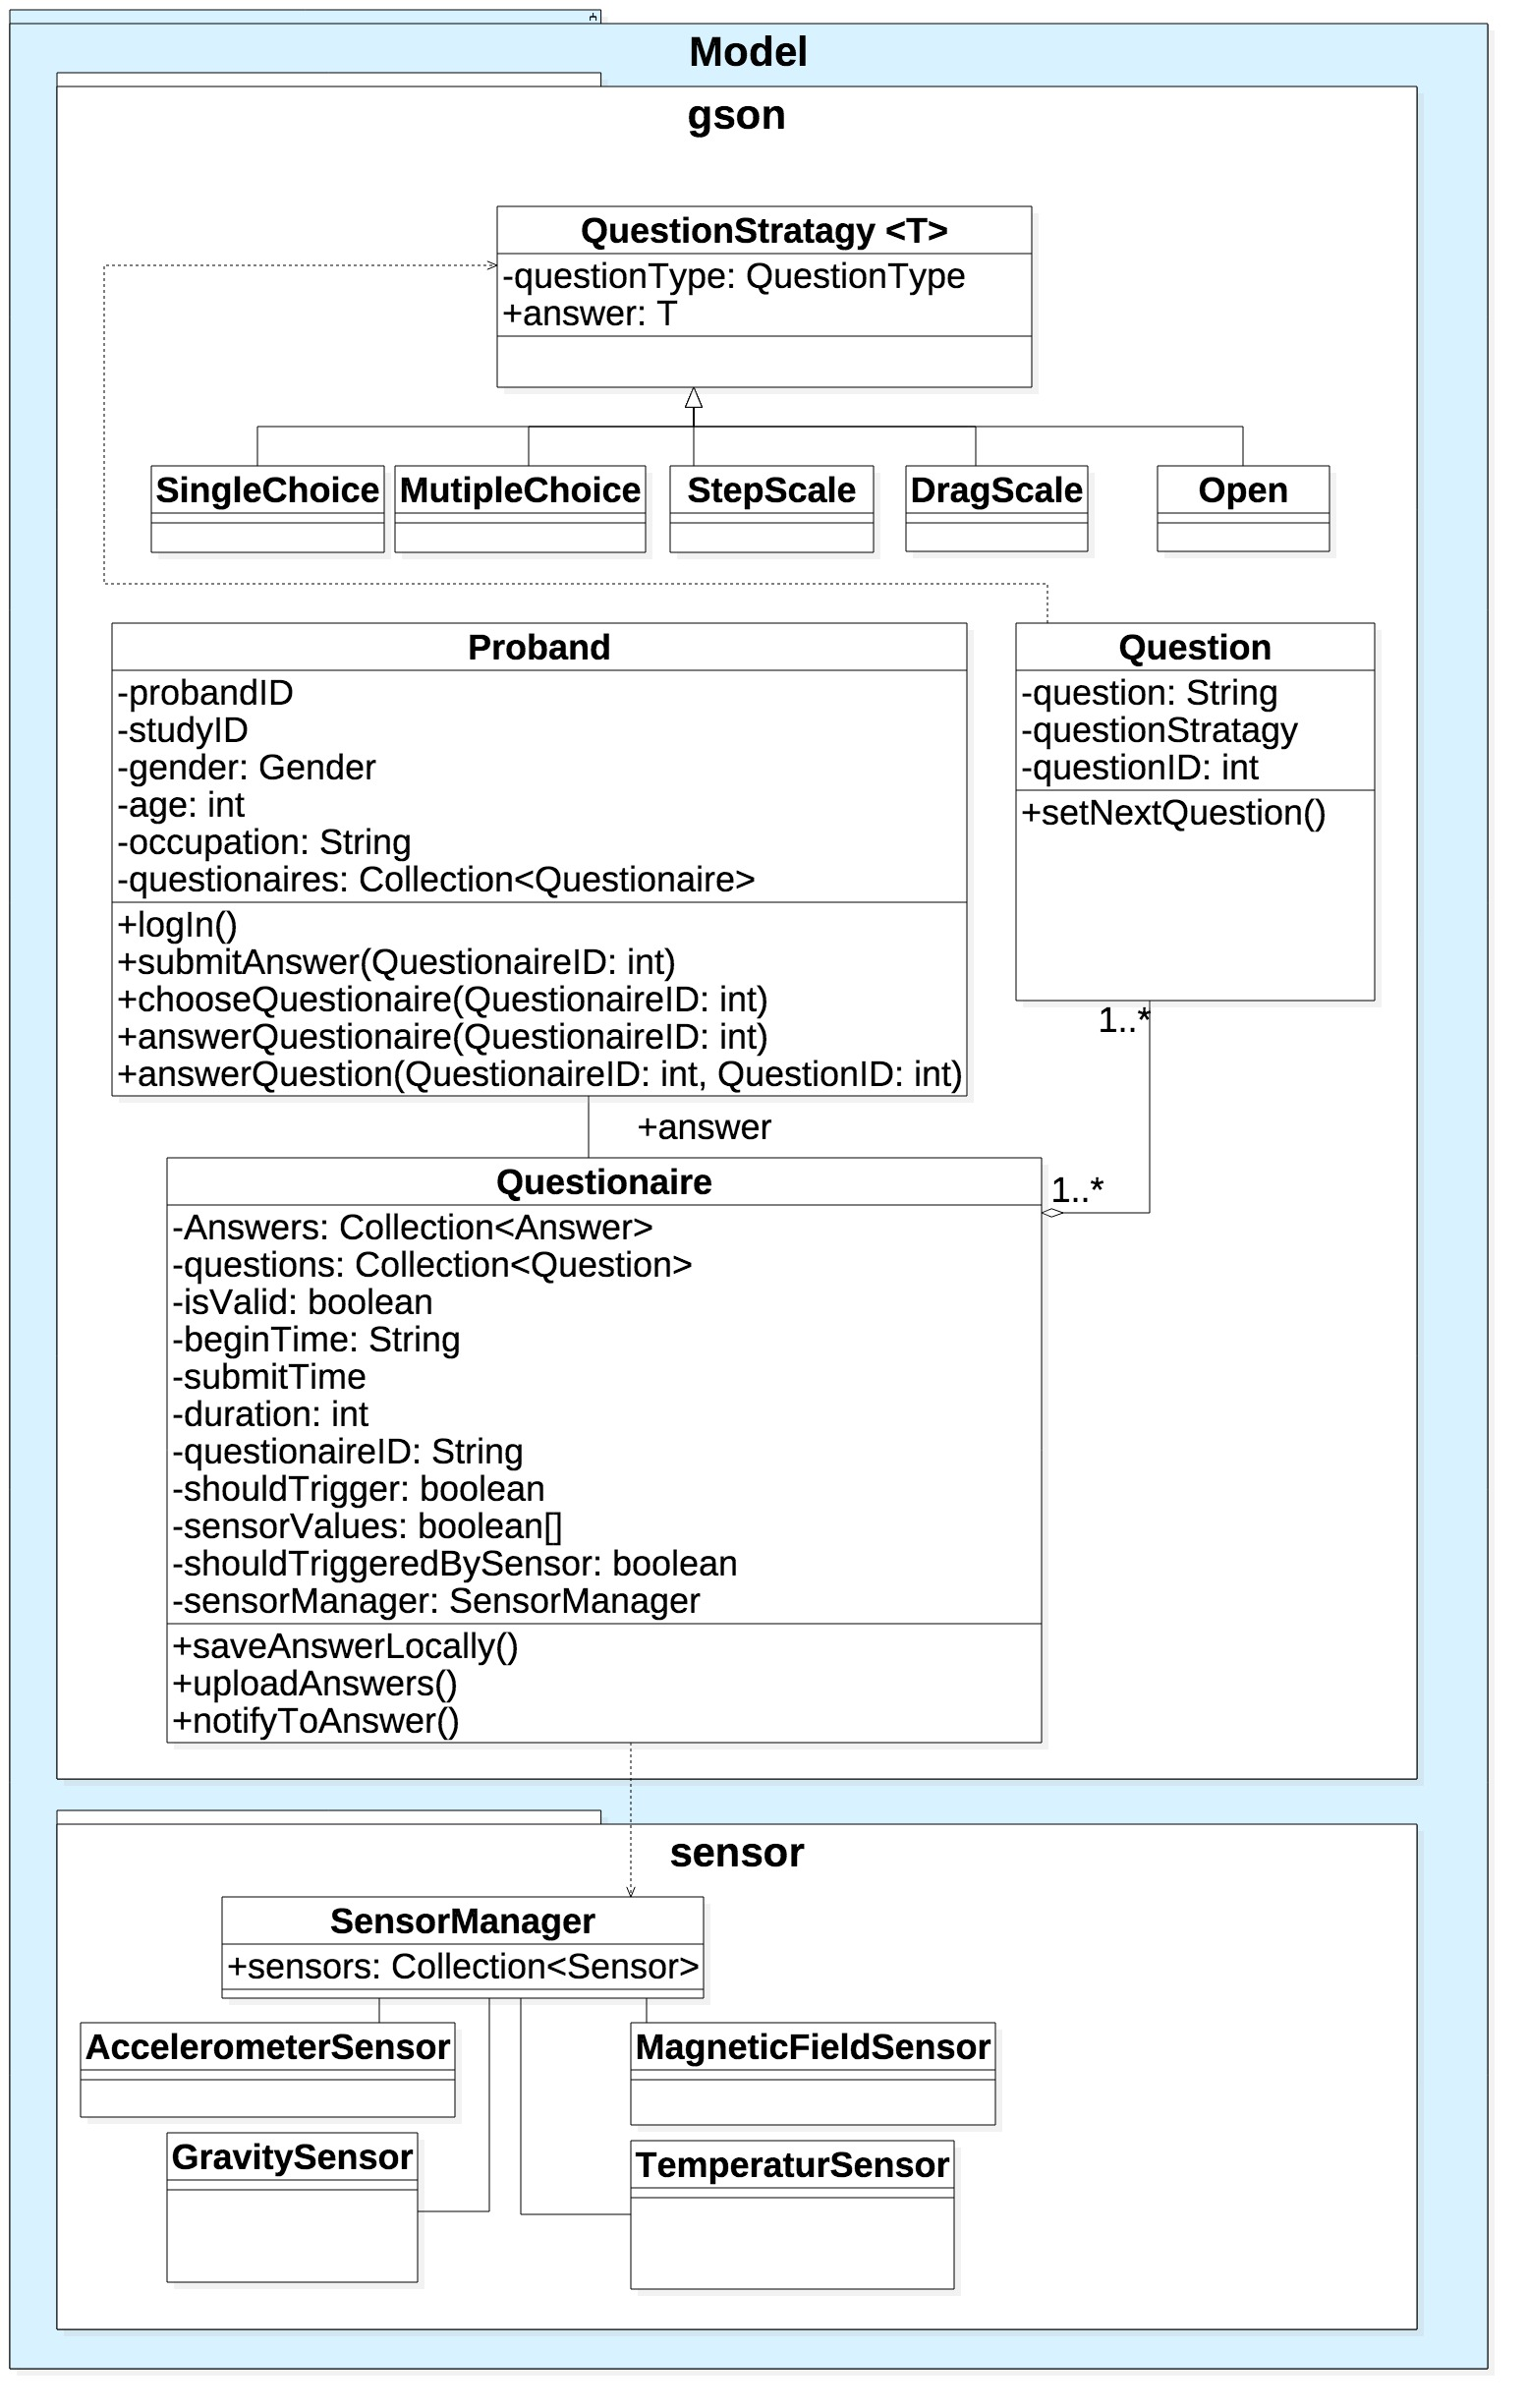
\includegraphics[scale=0.28]{Model.jpg}
                \caption{Model (Modelle)}
            \end{figure}


            \newpage
            \subsection{package \code{gson}}



                \subsubsection{class \code{Proband}}

                    \begin{enumerate}
                        \item Attribute
                            \begin{itemize}
                                \item \code{probandID:String}
                                \item \code{studyID:String}
                                \item \code{gender:Gender}
                                \item \code{age:int}
                                \item \code{occupation:String}
                                \item \code{questionnaires:Collection<Questionnaire>}
                            \end{itemize}
                        \item Methoden
                            \begin{itemize}
                                \item \code{login()}
                                \item \code{submitAnswer(QuestionID:String)}
                                \item \code{chooseQuestionnaire(QuestionnaireID:String):Questionnaire}
                                \item \code{answerQuestionniare(QuestionnaireID:String)}
                                \item \code{answerQuestion(QuestionnaireID:String, QuestionID:String)}
                                \item setters und getters für alle Attribute
                            \end{itemize}
                    \end{enumerate}



                \subsubsection{class \code{Questionnaire}}

                    \begin{enumerate}
                        \item Attribute
                            \begin{itemize}
                                \item \code{questions:Collection<Question>}
                                \item \code{isValid:boolean}
                                \item \code{beginTime:String}
                                \item \code{duration:int}
                                \item \code{QuestionnaireID:String}
                                \item \code{shouldTrigger:boolean}
                                \item \code{sensorValues:boolean[]}
                                \item \code{shouldTriggeredBySensor:booelan}
                                \item \code{sensorManager:SensorManager}
                            \end{itemize}
                        \item Methoden
                            \begin{itemize}
                                \item \code{saveAnswerLocally()}
                                \item \code{uploadAnswer(serverAddress:String)}
                                \item \code{notifyToAnsewr()}
                                \item setters und getters für alle Attribute
                            \end{itemize}
                    \end{enumerate}

                \subsubsection{class \code{Question}}

                    \begin{enumerate}
                        \item Attribute
                            \begin{itemize}
                                \item \code{question:String}
                                \item \code{questionType: QuestionStrategy}
                                \item \code{questionID: String}
                                \item \code{nextQuestionID: String}
                            \end{itemize}
                        \item Methoden
                            \begin{itemize}
                                \item setters und getters für alle Attribute
                            \end{itemize}
                    \end{enumerate}

                \subsubsection{abstract class \code{QuestionStrategy<T>}} %super abstract class

                    Hier wird Entwurfsmuster Stagtegie (eng: Strategy) eingesetzt, indem \code{QuestionStrategy} als Aggregation von \code{Question} und gleichzeitig als Oberklasse (eng: super class) von \code{SingleChoice}, \code{MutipleChoice}, \code{StepScale}, \code{DragScale} und \code{TextAnswer} gesetzt wird.
                    \begin{enumerate}
                        \item Attribute
                            \begin{itemize}
                                \item \code{answer:T}\\
                                    Generische Programmierung (eng:Generic) wird für attribute \code{answer} angewandet, da der Datentyp von Attribute \code{answer} in vershiedener Unterlasse von \code{QuestionStrategy} unterschiedlich sein sollte.
                                % \item \code{}
                                % \item \code{}
                            \end{itemize}
                        \item Methoden
                            \begin{itemize}
                                \item setters und getters für alle Attribute
                            \end{itemize}
                        \item Unterklasse\\
                            Laut Pflichtenheft gibt es fünf Fragearten. Deswegen gibt es fünf Unterklassen:
                            \begin{itemize}
                                \item class \code{SingleChoice}
                                \item class \code{MultipleChoice}
                                \item class \code{StepScale}
                                \item class \code{DragScale}
                                \item class \code{TextAnswer}
                            \end{itemize}
                    \end{enumerate}


            \subsection{package \code{Sensor}}
            \begin{figure}[H]
                \centering
                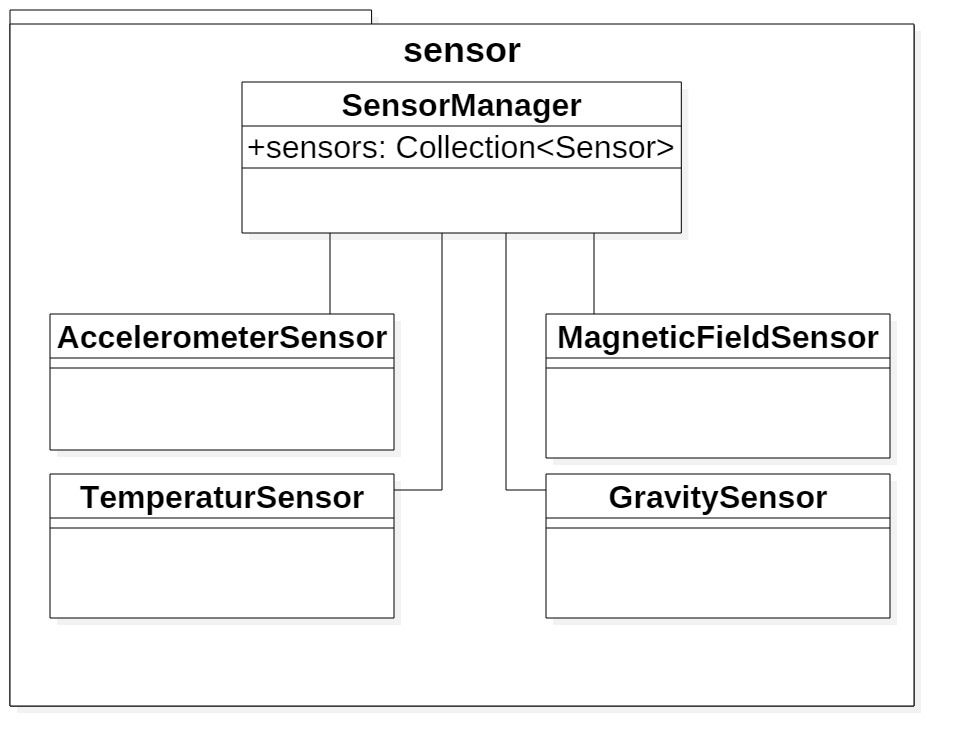
\includegraphics[scale = 0.5]{ClassDiagramAppSensor.jpg}
                \caption{Klassendiagramm für Sensoren in der Android Applikation }
            \end{figure}
                \subsubsection{class \code{SensorManager}}
                Diese Klasse ist einer Manager aller Sensoren, die in diesem Fragebogen bunutzt werden.
                \begin{enumerate}
                  \item Attribute
                    \begin{itemize}
                      \item \code{sensors:Collection<Sensor>}
                    \end{itemize}
                \end{enumerate}
                \subsubsection{class \code{AccelerometerSensor}}
                Diese Klasse handelt es sich um den Sensor über Beschleunigung.
                \subsubsection{class \code{GravitySensor}}
                Diese Klasse handelt es sich um den Sensor über Gravitation.
                \subsubsection{class \code{MagneticFeldSensor}}
                Diese Klasse handelt es sich um den Sensor über Magnetfeld.
                \subsubsection{class \code{TemperatureSensor}}
                Diese Klasse handelt es sich um den Sensor über Temperatur.
                


        \section{View}

            % provided by android


        \section{Control}
         Der Teil Model besteht aus zwei Pakete: activity und fragment.
            \begin{figure}[H]
                \centering
                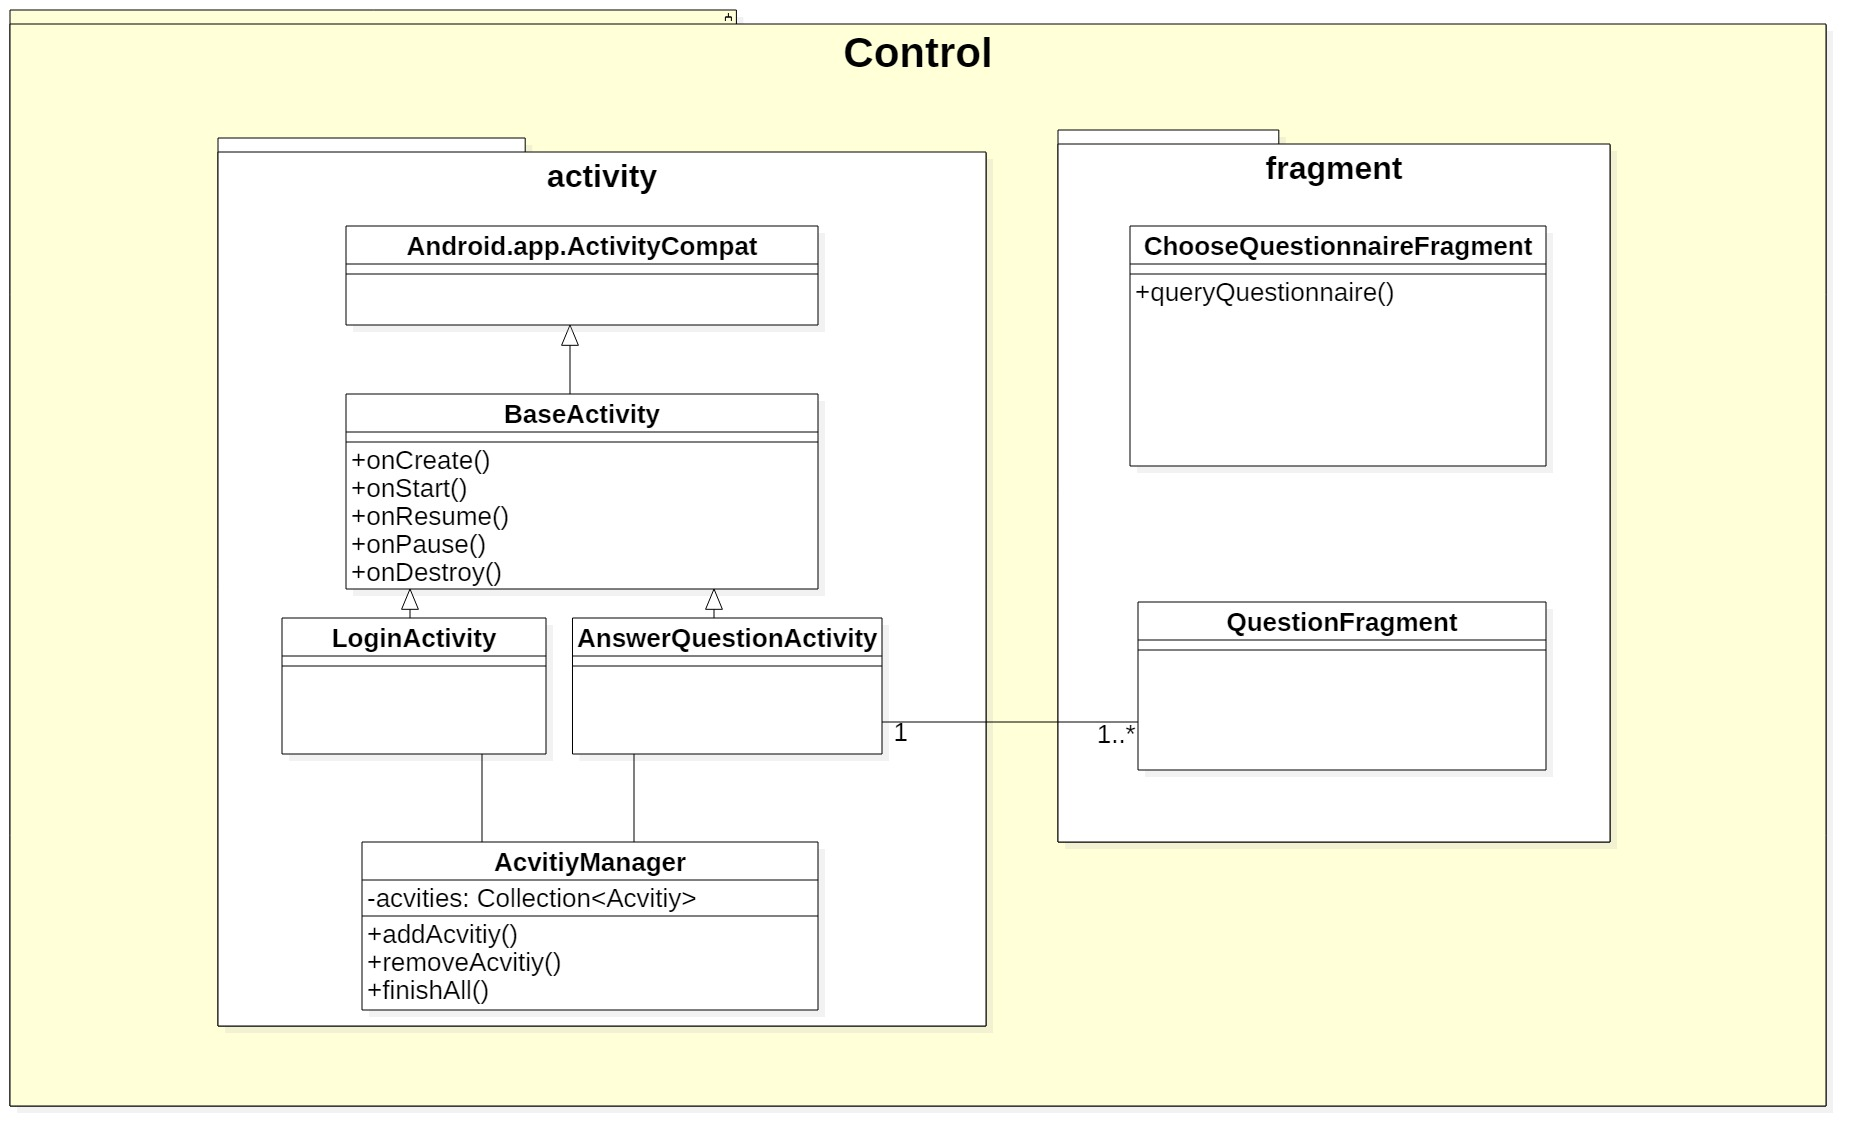
\includegraphics[scale = 0.3]{ControlClassDiagram(Android).jpg}
                \caption{Klassendiagramm für Control in der Android Applikation }
            \end{figure}

            \subsection{activity}

                \subsubsection{class \code{ActivityManager}}
                \begin{enumerate}
                \item Attribute
                     \begin{itemize}
                                \item \code{acvities: Collection<Acvitiy>}
                     \end{itemize}
                \item Methoden
                     \begin{itemize}
                                \item addAcvitiy()
                                \item removeAcvitiy()
                                \item finishAll()
                     \end{itemize}
                \end{enumerate}
                \subsubsection{class \code{BaseActivity}}
                \begin{enumerate}
                        \item Attribute
                        \item Methoden
                            \begin{itemize}
                                \item onCreate()
                                \item onStart()
                                \item onResume()
                                \item onPause()
                                \item onDestroy()
                            \end{itemize}
                \end{enumerate}
                \subsubsection{class \code{LogInActivity}}
                \begin{enumerate}
                        \item Attribute
                        \item Methoden
                \end{enumerate}
                \subsubsection{class \code{AnswerQuestionActivity}}
                 \begin{enumerate}
                        \item Attribute
                        \item Methoden
                \end{enumerate}

            \subsection{fragment}

                \subsubsection{class \code{ChooseQuestionnaireFragment}}
                \begin{enumerate}
                \item Attribute
                \item Methoden
                     \begin{itemize}
                                \item queryQuestionnaire()
                     \end{itemize}
                \end{enumerate}
                
                \subsubsection{class \code{QuestionFragment}}
                 \begin{enumerate}
                        \item Attribute
                        \item Methoden
                \end{enumerate}

        \section{Hilfpaket}




            \subsection{package \code{service}}

                \subsubsection{AutoDownloadService}

                \subsubsection{AutoUploadService}

            \newpage
            \subsection{package \code{util}}

                \vspace*{3cm}
                \begin{figure}[H]
                    \centering
                    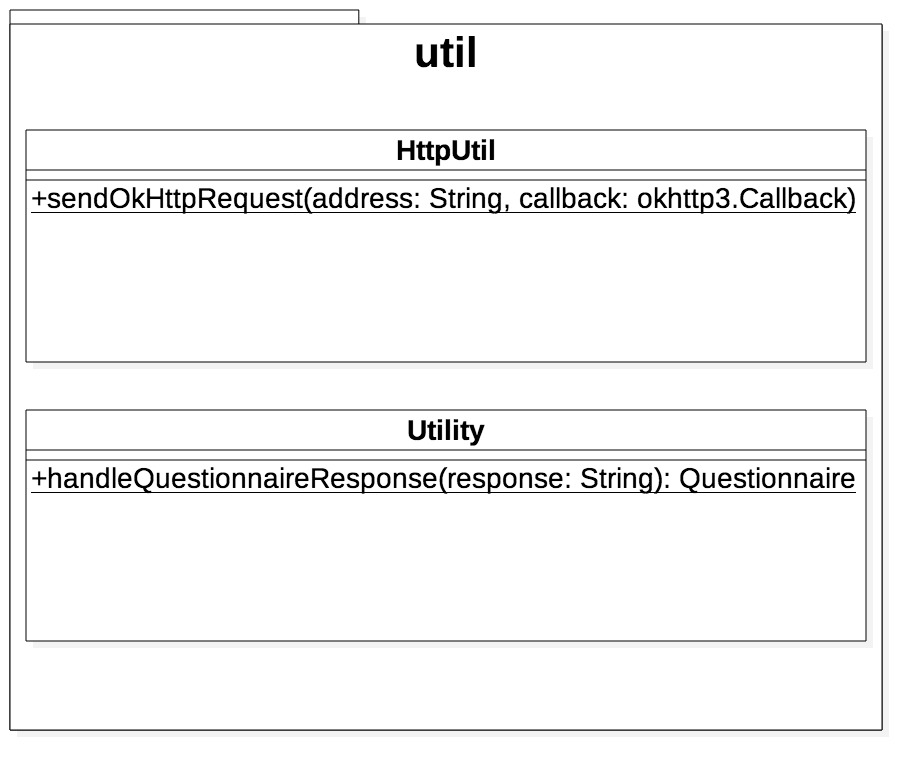
\includegraphics[scale = 0.5]{util.jpg}
                    \caption{package \code{util}}
                \end{figure}

                \subsubsection{class \code{HttpUtil}}

                    Diese Klasse ist zuständig für die Kommunikation zwischen Android-App und Server, indem wir die http-Framework OkHttp\footnote{http://square.github.io/okhttp/} verwenden.

                    \begin{enumerate}
                        \item Attribute
                        \item Methoden
                            \begin{itemize}
                                \item \code{static sendOkHttpRequest(address:String, callback:okhttp3.Callback)}
                            \end{itemize}
                    \end{enumerate}

                \subsubsection{class \code{Util}}

                    Diese Klasse bietet einige zweckmäßige Funktionen an, z.B. Analysierung der  von Server zurückgegebene Daten.

                    \begin{enumerate}
                        \item Attribute
                        \item Methoden
                            \begin{itemize}
                                \item \code{static handleQuestionnaireResponse(response:String):Questionnaire}\\
                                Diese Method analysiert die von Server zurückgegebene json Daten und gibt \code{Questionnaire} Objekt zurück.
                            \end{itemize}
                    \end{enumerate}


    \glsaddall
    \printglossary

    % Abbildungsverzeichnis
    \listoffigures

\end{document}
